\subsection{Resampling Methods}

\noindent \textbf{Resampling methods}: techniques that involve repeatedly drawing samples from a training data and refitting the model on each (re)sample in order to obtain additional information about the fitted model.

\noindent Two Main Resampling Methods:

\begin{itemize}
    \item \textbf{Cross-Validation (CV)}: Used to estimate test error and select tuning parameters.
    \item \textbf{Bootstrap}: Used primarily to assess variability, e.g., standard errors and confidence intervals
\end{itemize}

\subsubsection{Training error VS test error}

\indent 

\noindent\textbf{Training error}: the performance metric applied to the observations used to train the model.

\noindent\textbf{Test error}: the average error when applying a model to predict the response on new (test) observations that were not used in the training of the model.

\bigskip

Training error is usually very different in magnitude to the test error. Training error can underestimate the test error.

\subsubsection{Test set approach}

\indent 

\step Here, we randomly divide the available set of samples into two: a training set and a test set.

\step The model is fit on the training set, and the fitted model is used to predict the responses for the observations in the test set.

\step The resulting test-set error provides an estimate of the test error.

Typically assessed using:

\begin{itemize}
    \item \textbf{MSE}: in the case of a quantitative response (regression)
    \item \textbf{Misclassification rate}: in the case of a qualitative (discrete) response (classification)
\end{itemize}

The estimate of the test error can be highly variable, depending on precisely which observations are included in the training set and which observations are included in the test set.

In the test set approach, only a subset of the observations are used to fit the model. This suggests that the test set error may tend to overestimate the test error for the model fit on the entire data set.

\subsection{$k$-fold and repeated cross validation}

\subsubsection{$k$-fold cross validation}

\indent 

Widely used approach for estimating test error. Estimates can be used to select best model, and to give an idea of the test error of the final chosen model.

randomly divide the data into $k$ equal-sized parts and the procedure is repeated $k$ times. Each time, the first fold is treated as a test set, and the method is fit on the remaining $k-1$ folds. The $\text{MSE}_i$ is computed at each iteration. The $k$-fold CV estimate is computed by averaging these values:

\begin{align*}
    \text{CV}_{(k)} = \frac{1}{k}\sum_{i=1}^{k}\text{MSE}_i
\end{align*}

\subsubsection{Repeated Cross Validation}

\indent 

It repeats the $k$-fold CV process multiple times, each with different random splits. This helps to: provide a less biased CV test error estimate. provide the variance of the CV error. It comes with a \textbf{computational cost}.

\noindent\textbf{Other things you should do it within with CV loop}:

\begin{itemize}
    \item Feature selection
    \item Hyperparameter optimization
    \item Missing data imputation
\end{itemize}

\subsubsection{Model Selection}

\indent 

The reason for doing cross-validation is to evaluate the different models by estimating their performance on unseen data. If you need to choose between kNN, LDA, logistic regression, and SVM, then you can run each of these classification algorithms with cross-validation, and pick the one with the highest CV accuracy. But then, you can go back to use all the data to build a final model.

\subsection{Classification evaluation metrics}

\subsubsection{Confusion Matrix}

\begin{figure}[h]
    \centering
    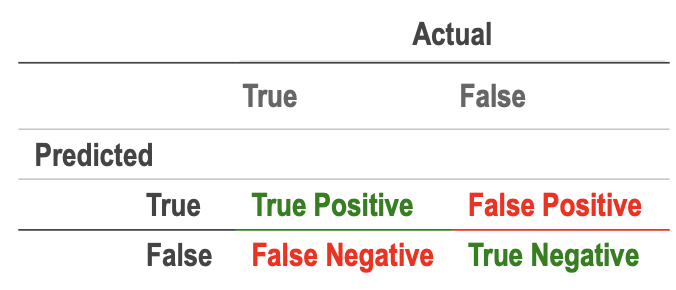
\includegraphics[width=0.6\linewidth]{Figure/Week 6/Confusion Matrix.png}
\end{figure}

\begin{itemize}
    \item \textbf{True positive}: positive class and predicted to be positive class.
    \item \textbf{False positive}: negative class but predicted to be positive class.
    \item \textbf{False negative}: positive class but predicted to be negative class.
    \item \textbf{True negative}: negative class and predicted to be negative class.
\end{itemize}

\subsubsection{Accuracy}

\begin{align*}
    \text{Accuracy} = \frac{\text{Number of Correct Predictions}}{\text{Total Number of Observations}} = \frac{TP+TN}{TP+TN+FP+FN}
\end{align*}

\noindent\textbf{Limitations of Accuracy}:

Ignores the type of error: Accuracy makes no distinction about the type of errors being made. In some cases, errors have unequal costs.

Not suitable for imbalanced data: If one class is dominant, predicting the majority class yields high accuracy but poor real performance.

\subsubsection{Alternatives}

\begin{align*}
    \text{Racall (Sensitivity)} & = \frac{TP}{TP+FN} = \frac{TP}{P}\\
    \text{Specificity} & = \frac{TN}{TN+FP} = \frac{TN}{N}\\
    \text{Precision} & =\frac{TP}{TP+FP}\\
    \text{F1} & = \frac{2\times\text{Precision}\times\text{Recall}}{\text{Precision}+\text{Recall}}\text{(Harmonic mean)}\\
    \text{GM} & =\sqrt{\text{Precision} \times \text{Recall}}\text{(Geometric mean)}
\end{align*}

\subsubsection{Receiver Operating Characteristic (ROC) Curve}

\indent 

\noindent\textbf{ROC curve}: a graphical tool used to evaluate the performance of a binary classifier.

It plots the Sensitivity against the False Positive Rate (1 - Specificity) at various threshold settings. Each point on the ROC curve corresponds to a different decision threshold. The closer the curve is to the top-left corner, the better the model.

It helps compare classification models. Useful when classes are imbalanced.

\noindent \textbf{Area Under the Curve (AUC)}: summarises the overall performance.

\begin{itemize}
    \item \textbf{$\text{AUC} = 1$}: Perfect model
    \item \textbf{$\text{AUC} = 0.5$}: No better than random guessing
\end{itemize}

\subsection{Multi-class classfication}

\indent 

Performance measured like precision, recall, $\text{F1}$, and AUC may be generalised to classification problems with more than 2 labels.